


\begin{frame}
\frametitle{Load Imbalance}
\begin{itemize}
\item Performance limited by difference between most-loaded processor and overall average.\\
\only<1>{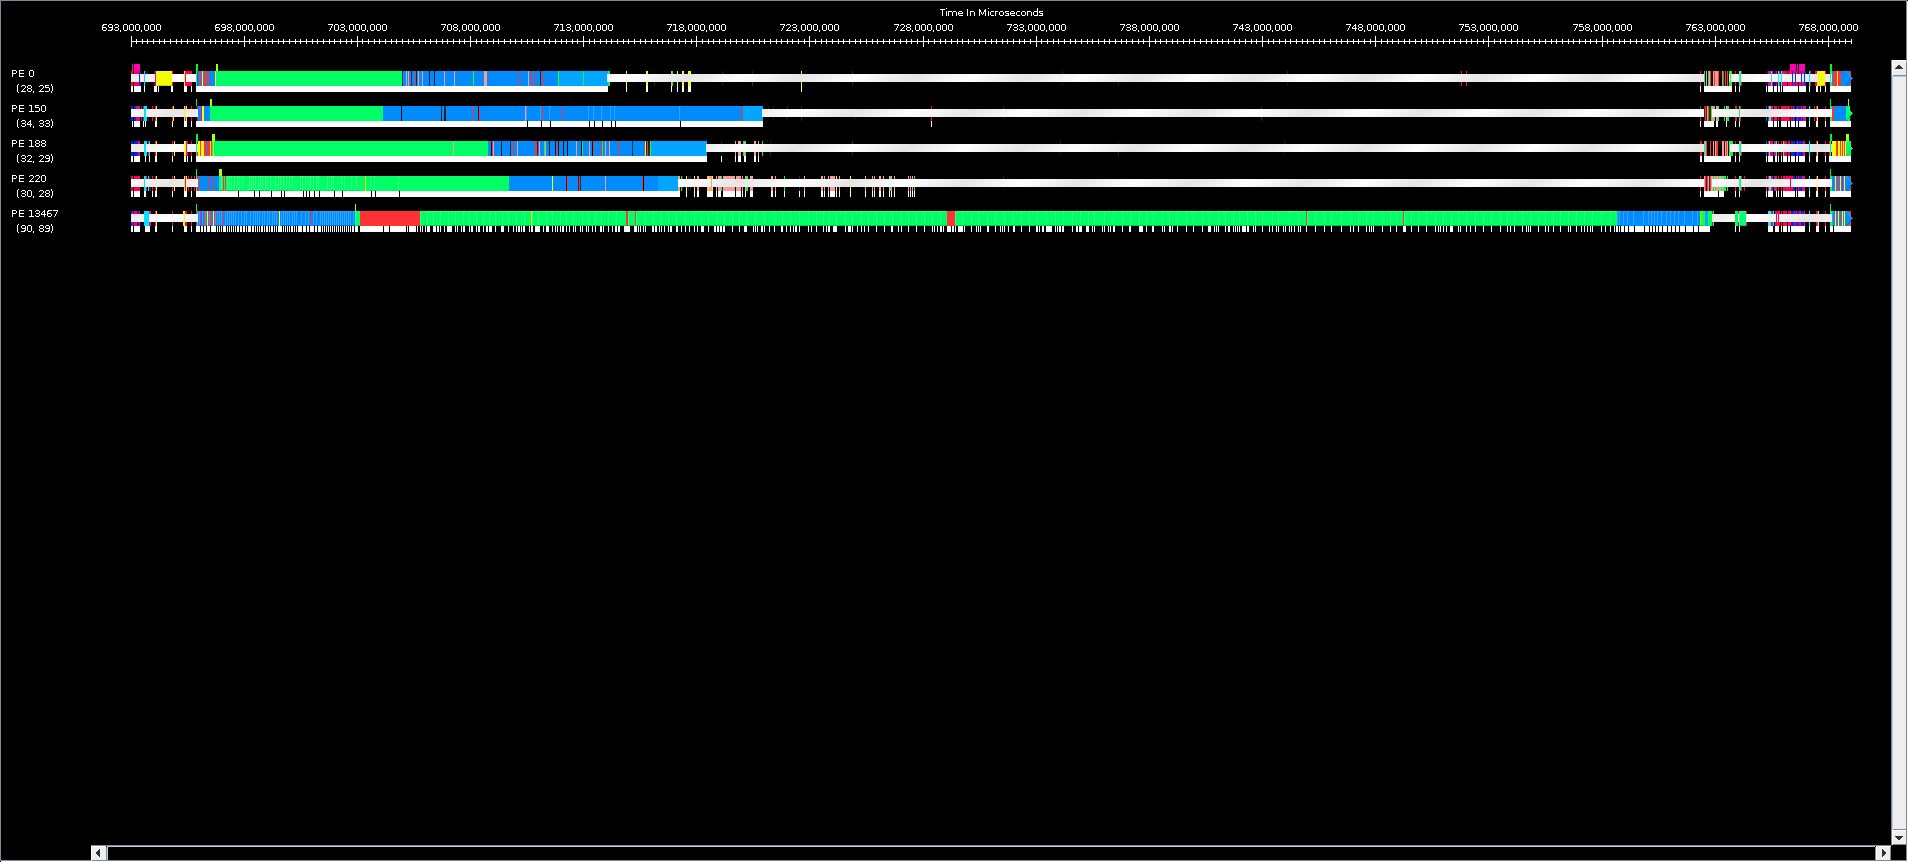
\includegraphics[width=0.8\textwidth]{../figures/changa_imbalance.png}}
\pause
\item Causes vary in severity, time scale, nature
\pause
\item Response must suit causes, other application concerns, system scale
\end{itemize}
\end{frame}


\begin{frame}[fragile]
\frametitle{Load Imbalance: Crack Propagation}
\begin{columns}
\begin{column}{0.5\textwidth}
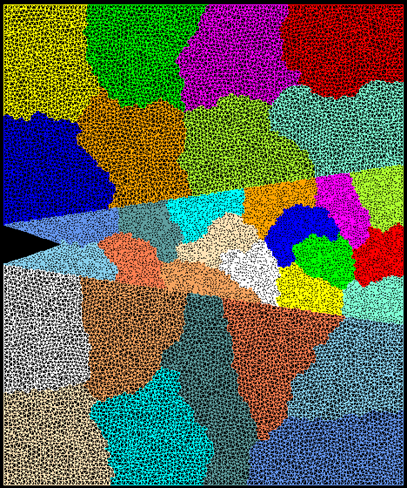
\includegraphics[width=\textwidth]{../figures/chunkGraph16}
\end{column}
\begin{column}{0.5\textwidth}
Decomposition into 16 chunks using Metis. The middle area contains cohesive elements.

As computation progresses, crack propagates, and new elements are added, leading to more complex computations in some chunks

Picture: S. Breitenfeld and P. Geubelle
\end{column}
\end{columns}
\end{frame}

\begin{frame}[fragile]
\frametitle{Load Balancing Crack Propagation}
\begin{centering}
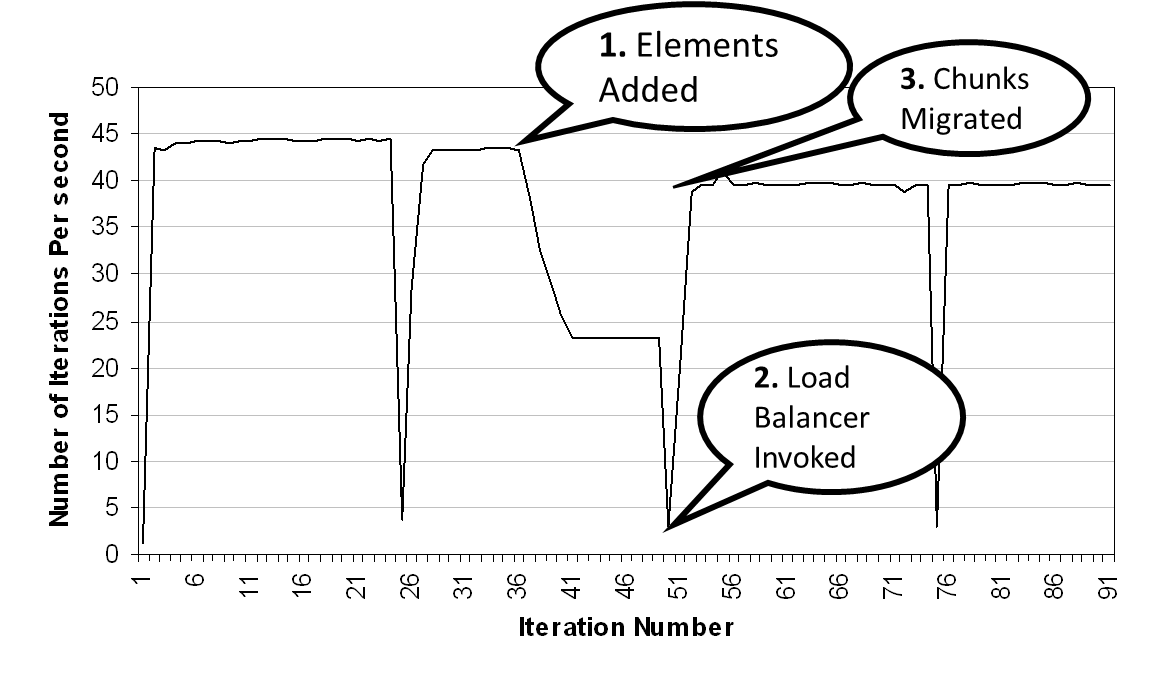
\includegraphics[width=0.8\textwidth]{../figures/LButilizationCrackPropWithAnnotation}
\end{centering}
\begin{block}{Sudden, severe shift in load suggests comprehensive rebalancing}
Link-time: \texttt{-balancer GreedyLB} or \texttt{-balancer MetisLB} \\
Run-time: \texttt{+balancer FooLB}
\end{block}
\end{frame}


\begin{frame}
\frametitle{Load Balancing Adaptive Mesh Refinement for solving PDEs}
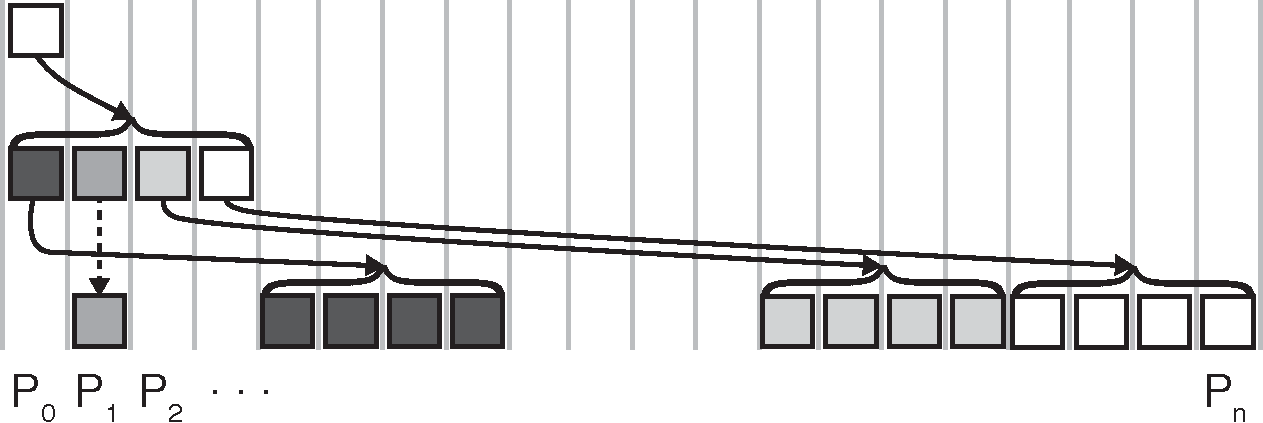
\includegraphics[width=0.9\textwidth]{../figures/amr_mapping.pdf}\\
Load changes gradually and incrementally, suggesting localized strategies
\end{frame}


\begin{frame}
\frametitle{Load Balancing Adaptive Mesh Refinement for solving PDEs}
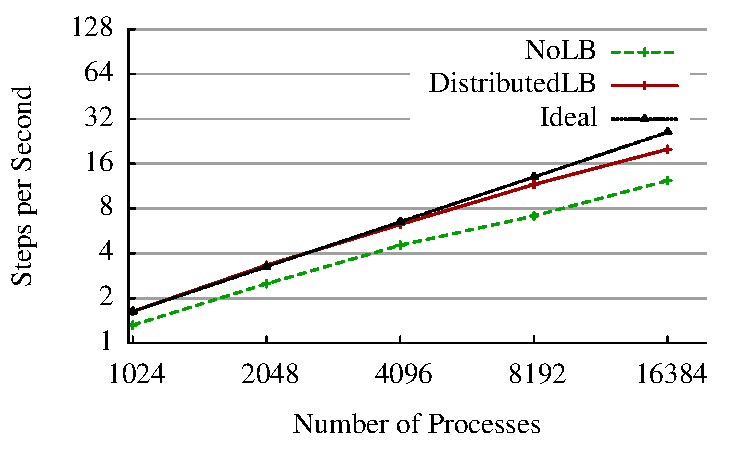
\includegraphics[width=0.9\textwidth]{../figures/amr_scaling_distlb.pdf}
\end{frame}

\begin{frame}
\frametitle{Load Imbalance: Adaptive Response}
\begin{itemize}
\item When to run load balancer? \pause When imbalance hurts (worse than the cost)!
\end{itemize}
\only<2>{
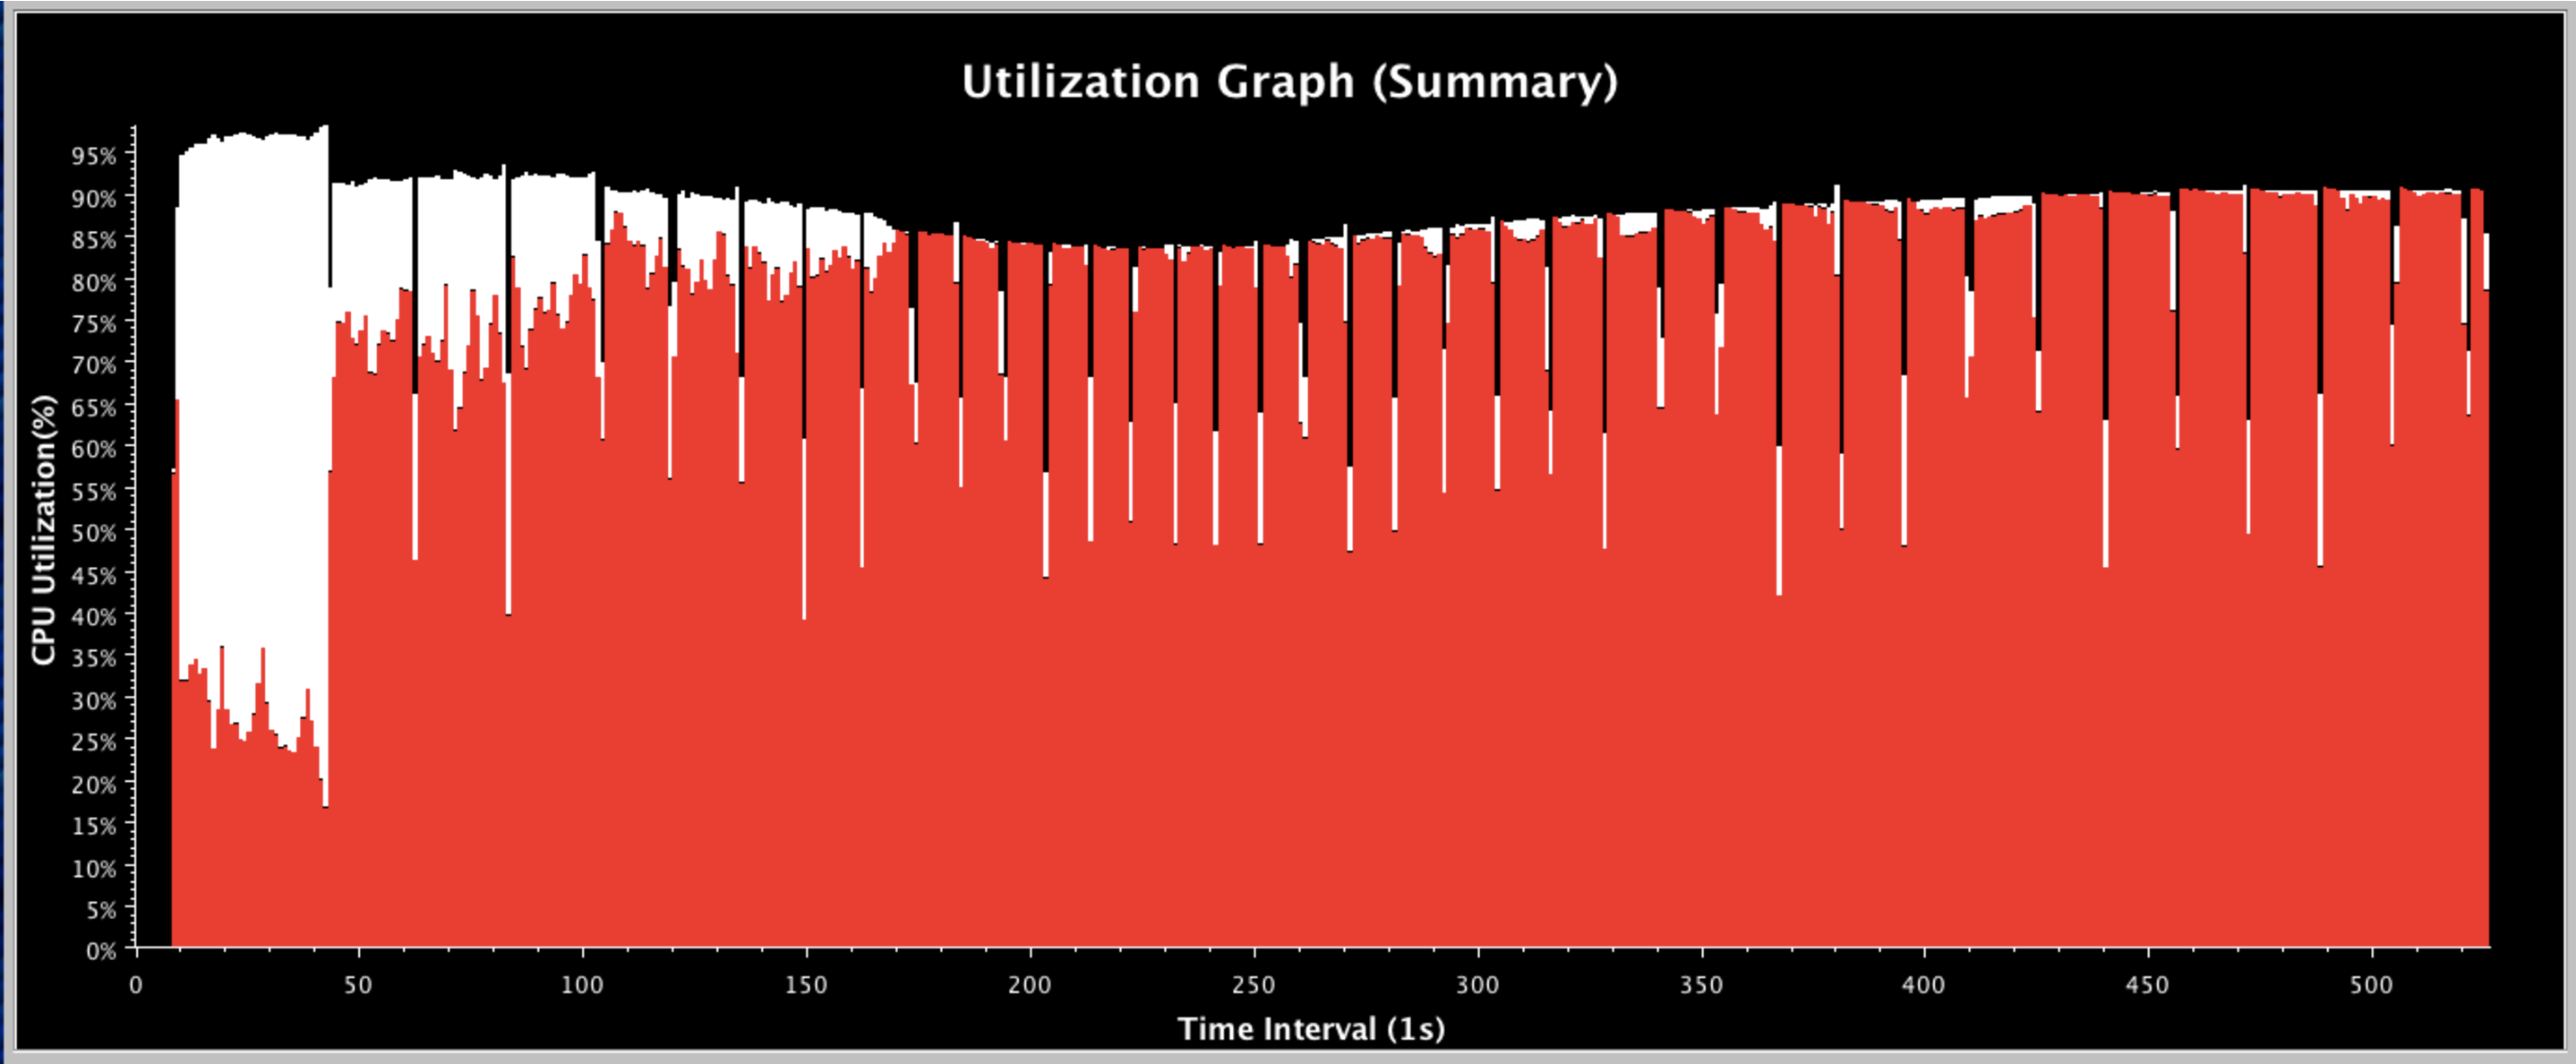
\includegraphics[width=0.5\textwidth]{../figures/figs_frac_titan_lb300_vp4k_64_proj.pdf}
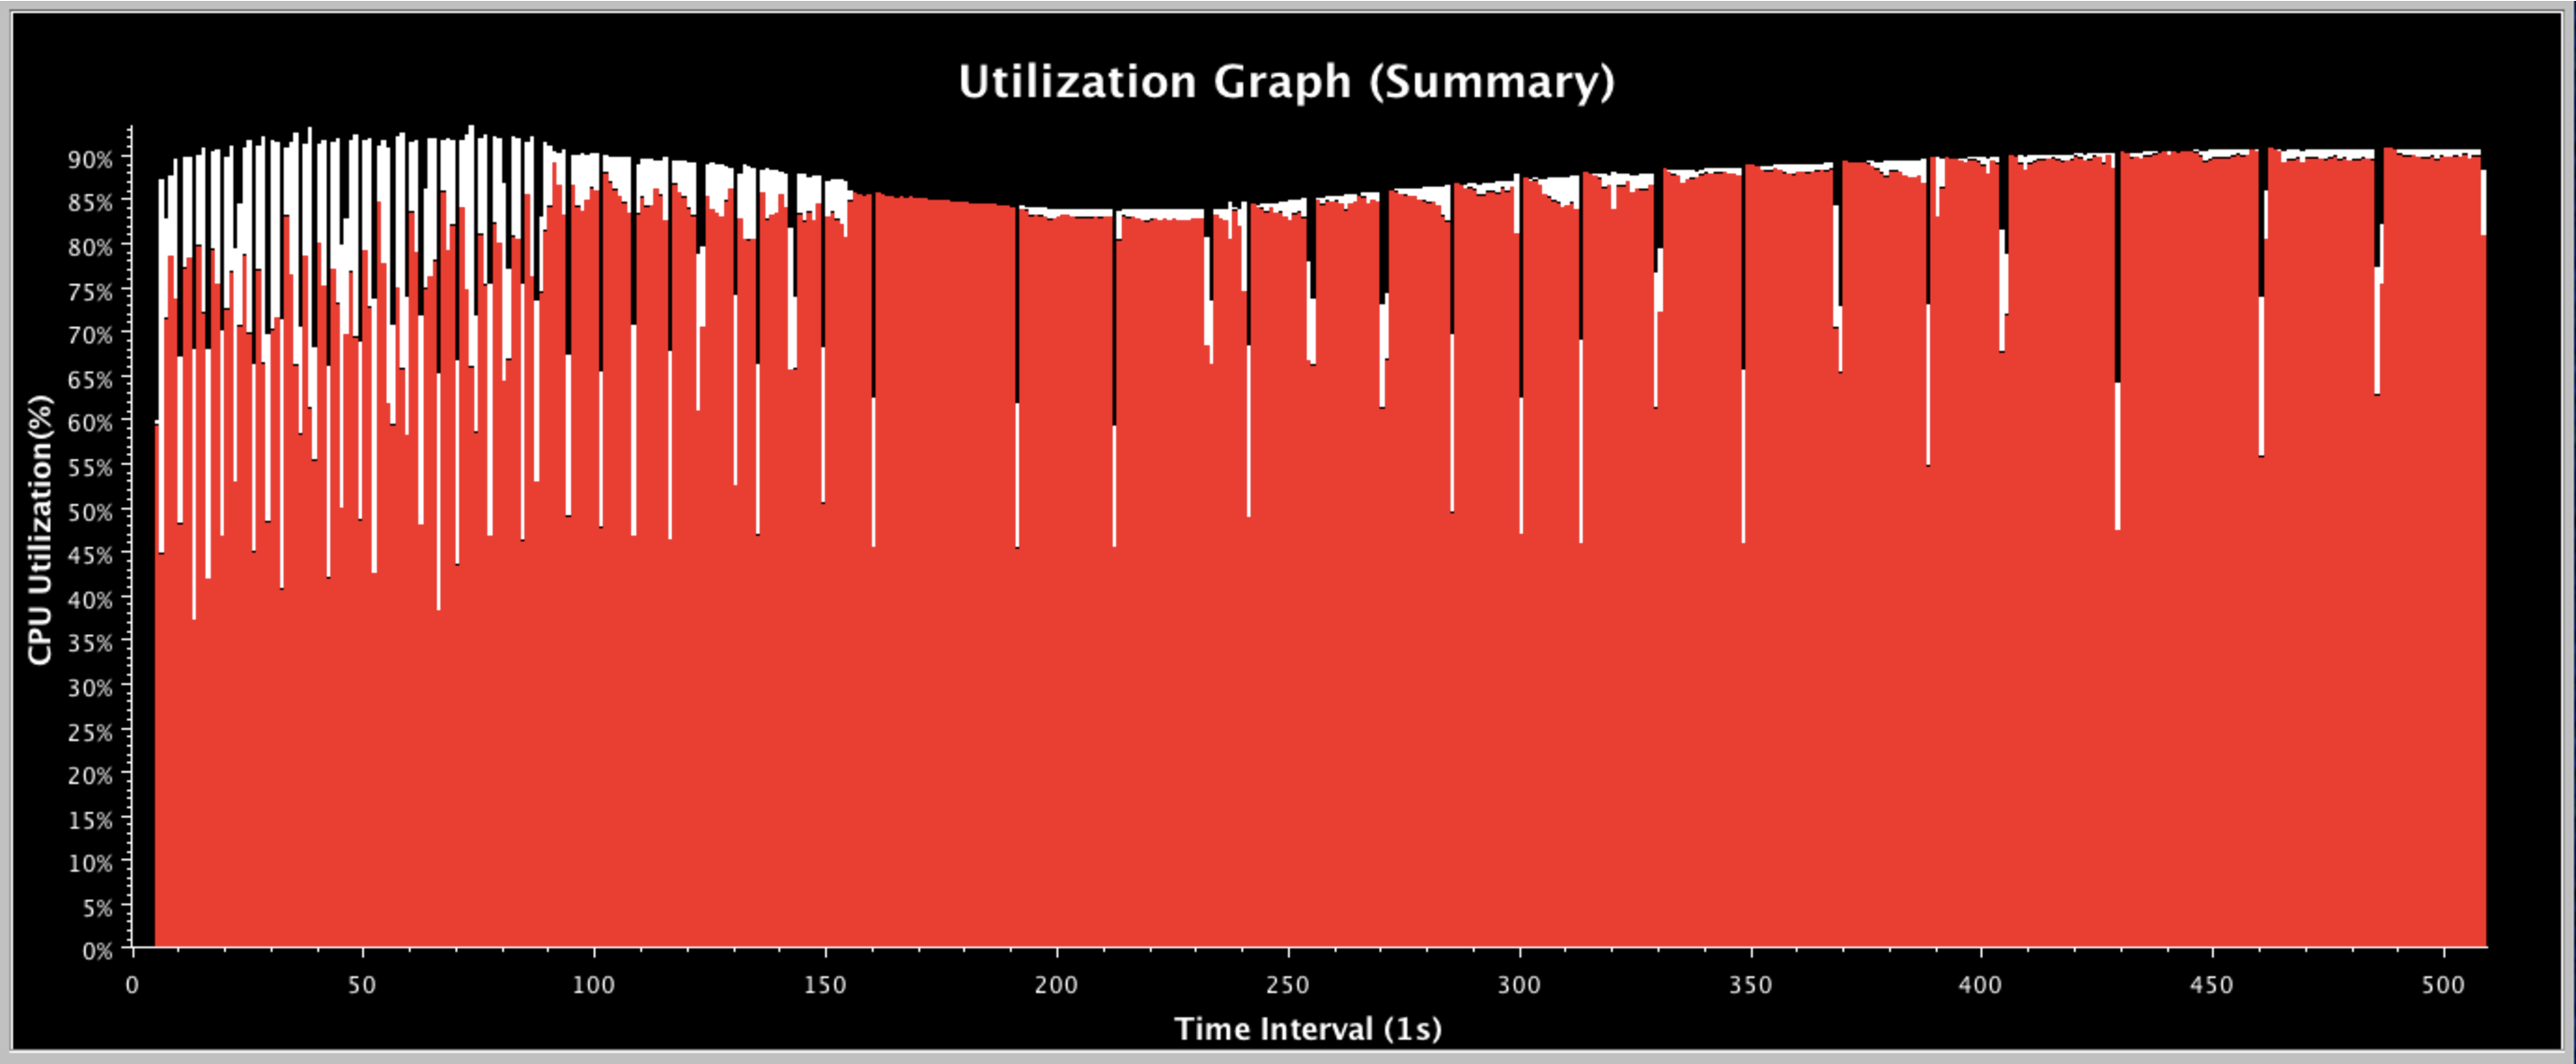
\includegraphics[width=0.5\textwidth]{../figures/figs_frac_titan_meta_vp4k_64_proj.pdf}
\begin{block}{How to activate?}
\texttt{./pgm argsA argsB argsC +MetaLB}
\end{block}
}
\end{frame}

\begin{frame}
\frametitle{Load Imbalance: Adaptive Response}
\begin{itemize}
\item When to run load balancer? When imbalance hurts (worse than the cost)!
\item When to allow migration? \pause When imbalance hurts (worse than the cost)!
\end{itemize}
\only<2>{
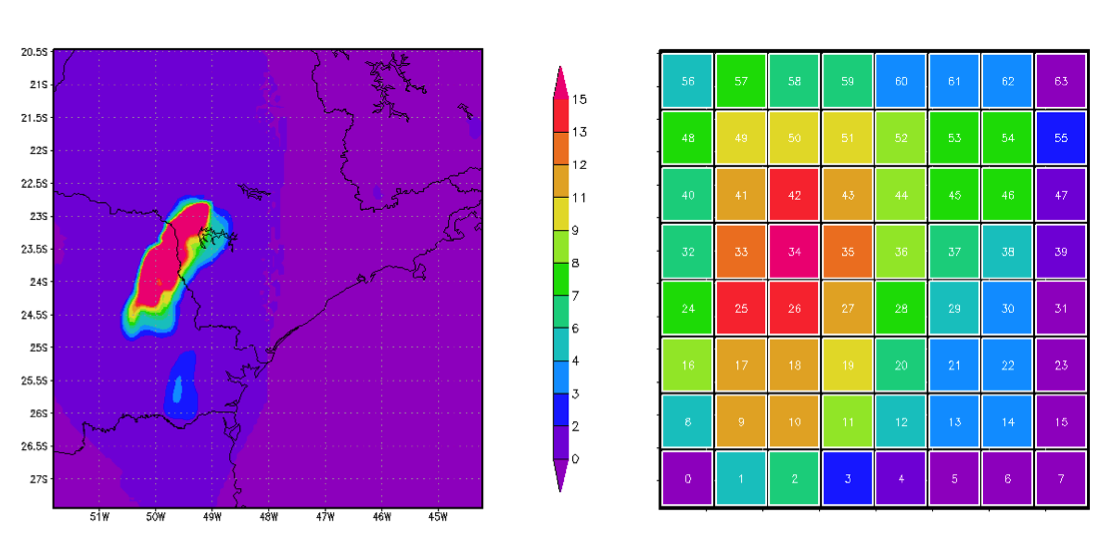
\includegraphics[width=0.9\textwidth]{../figures/bramsVisual.png}
}
\end{frame}
